\documentclass{scrreprt}

\usepackage[utf8]{inputenc}
\usepackage{enumerate}
\usepackage{ngerman}
%\usepackage[german]{babel}

\usepackage{amsmath}
\usepackage{amsfonts}
\usepackage{amssymb}
\usepackage{amsthm}
\usepackage{mathtools}

\usepackage{pgf,tikz}
\usepackage{mathrsfs}
\usetikzlibrary{arrows} 

\usepackage[hidelinks]{hyperref}

\makeatletter
\def\moverlay{\mathpalette\mov@rlay}
\def\mov@rlay#1#2{\leavevmode\vtop{%
   \baselineskip\z@skip \lineskiplimit-\maxdimen
   \ialign{\hfil$\m@th#1##$\hfil\cr#2\crcr}}}
\newcommand{\charfusion}[3][\mathord]{
    #1{\ifx#1\mathop\vphantom{#2}\fi
        \mathpalette\mov@rlay{#2\cr#3}
      }
    \ifx#1\mathop\expandafter\displaylimits\fi}
\renewcommand*\env@matrix[1][*\c@MaxMatrixCols c]{%
  \hskip -\arraycolsep
  \let\@ifnextchar\new@ifnextchar
  \array{#1}}
\makeatother

\newcommand{\NN}{\mathbb{N}}
\newcommand{\ZZ}{\mathbb{Z}}
\newcommand{\QQ}{\mathbb{Q}}
\newcommand{\RR}{\mathbb{R}}
\newcommand{\CC}{\mathbb{C}}
\newcommand{\cupdot}{\charfusion[\mathbin]{\cup}{\cdot}}
\newcommand{\bigcupdot}{\charfusion[\mathop]{\bigcup}{\cdot}}


\begin{document}

	\title{Analysis 1}
 	\author{Dominic Zimmer, Alexander Yongsap\\in Kollaboration mit Jesko Dujmovic und Pascal Weber}
 	\subtitle{Übungsblatt 9, Abgabe}
 	\publishers{Übungsgruppe: Rami Ahmad}
  	\maketitle 

	%see http://www.namsu.de/Extra/strukturen/Inhaltsverzeichnis.html

\section*{Aufgabe 1}
\begin{enumerate}[(a)]
\item
    Zu zeigen: Für alle $z_1 = (r_1, i_1)$, $z_2 = (r_2, i_2)$, $z_3 = (r_3, i_3)$ gilt:
    \begin{align*}
        z_1 \cdot (z_2 \cdot z_3) & = (r_1, i_1) \cdot ( r_2  r_3 - i_3  i_2, r_2  i_3 + r_3  i_2 )\\
        & = (r_1 \cdot (r_2  r_3 - i_2  i_3) - i_1 \cdot (r_2  i_3 + r_3  i_2), r_1 \cdot (r_2  i_3 + r_3  i_2) + i_1 \cdot (r_2  r_3 - i_2  i_3))\\
        & = (r_1 r_2 r_3 - r_1 i_2 i_3 - i_1 r_2 i_3 - i_1 r_3 i_2, r_1 r_2 i_3 + r_1 r_2 i_2 + i_1 r_2 r_3 - i_1 i_2 i_3)\\
        & = ((r_1 r_2 - i_1 i_2) \cdot r_3 - (r_1 i_2 + i_1 r_2) \cdot i_3, (r_1 r_2 - i_1 i_2) \cdot i_3 + (r_1 i_2 + i_1 r_2) \cdot r_2)\\
        & = (r_1 r_2 - i_1 i_2, r_1 i_2 + i_1 r_2) \cdot (r_3, i_3)\\
        & = (z_1 \cdot z_2) \cdot z_3   
    \end{align*}
\item
    Zu zeigen: Für alle $z_1 = (r_1, i_1)$, $z_2 = (r_2, i_2)$, $z_3 = (r_3, i_3)$ gilt:
    \begin{align*}
        z_1 \cdot (z_2 + z_3) & = (r_1, i_1) \cdot (r_2 + r_3, i_2 + i_3)\\
        & = (r_1 \cdot (r_2 + r_3) - i_1 \cdot (i_2 + i_3) , r_1 \cdot (i_2 + i_3) + i_1 \cdot (r_2 + r_3))\\
        & = (r_1 r_2 + r_1 r_3 - i_1 i_2 - i_1 i_3, r_1 i_2 + r_1 i_3 + i_1 r_2 + i_1 r_3)\\
        & = (r_1 r_2 - i_1 i_2, r_1 i_2 + i_1 r_2) + (r_1 r_3 - i_1 i_3, r_1 i_3 + i_1 r_3)\\
        & = (r_1, i_1) \cdot (r_2, i_2) + (r_1, i_1) \cdot (r_3, i_3)\\
        & = z_1 z_2 + z_1 z_3\\
    \end{align*}
\item
    Wir suchen ein Multiplikatives Inverses zu jedem $0 \neq z \in \CC$, so dass $z \cdot z^{-1} = (1,0)$. Komponentenweise ausmultipliziert ergibt dies zwei Gleichungen:
    \begin{align*}
        (1,0) & = z \cdot z^{-1} = (r, i) \cdot (r^{-1}, i^{-1}) = (r  \cdot r^{-1} - i \cdot i^{-1}, r \cdot i^{-1} + i\cdot r^{-1})
    \end{align*}
    Wir lösen das Gleichungssystem nun in den Variablen $r^{-1}$ und $i^{-1}$:
    \begin{align*}
        \begin{pmatrix}[cc|c]
            r & -i & 1\\
            i & r & 0\\
        \end{pmatrix}
        \leadsto
        \begin{pmatrix}[cc|c]
            r \cdot i & -i^2 & i\\
            r \cdot i & r^2 & 0\\
        \end{pmatrix}
        \leadsto
        \begin{pmatrix}[cc|c]
            r \cdot i & -i^2 & i\\
            0 & r^2 + i^2 & -i\\
        \end{pmatrix}
        \leadsto
        \begin{pmatrix}[cc|c]
            r \cdot i & -i^2 & i\\
            0 & 1 & \frac{-i}{r^2 + i^2}
        \end{pmatrix}
    \end{align*}
    Als Lösungen erhalten wir (mit dem Gaußalgorithmus):
    \begin{align*}
        r^{-1} = \frac{r}{r^2 + i^2} ~~~ i^{-1} = \frac{-i}{r^2 + i^2}\\
        \Rightarrow z^{-1} = \left(\frac{r}{r^2 + i^2},\frac{-i}{r^2 + i^2}\right)
    \end{align*}
\item
    Zu zeigen: Für alle $z_1 = (r_1, i_1)$, $z_2 = (r_2, i_2)$ gilt: 
    \begin{align*}
        \overline{z_1 \cdot z_2} & = \overline{(r_1, i_1) \cdot (r_2, i_2)}\\
        & = \overline{(r_1 r_2 - i_1 i_2, r_1 i_2 + r_2 i_1)}\\
        & = (r_1 r_2 - i_1 i_2, - r_1 i_2 - r_2 i_1)\\
        & = (r_1, -i_1) \cdot (r_2, -i_2)\\
        & = \overline{(r_1, i_1)} \cdot \overline{(r_2, i_2)}\\
        & = \overline{z_1} \cdot \overline{z_2}
    \end{align*}
\end{enumerate}

\section*{Aufgabe 2}
Bringen sie die folgenden Komplexen Terme auf die Form $a + b i$, $(a,b) \in \RR^2$.
\begin{enumerate}[(a)]
\item
    \begin{align*}
        (1 + 2i) \cdot (3-i) & = (1 \cdot 3 - 2i \cdot i) + (2i \cdot 3 - 1 \cdot i)\\
        & = 5 + (5)i
    \end{align*}
\item
    \begin{align*}
        \frac{2}{i^3} & = \frac{2\cdot i}{i^4} = 2i
    \end{align*}
\item
    \begin{align*}
        \frac{1+i}{1-i} = \frac{(1+i)^2}{1 + 1} = \frac{1 + 2i - 1}{2} = i
    \end{align*}
\item
    \begin{align*}
        \frac{(3 + 2i)(7 - 3i)}{2 + 4i} = \frac{(15-23i)(2-4i)}{(2+4i)(2-4i)} = \frac{-62 - 106i}{-20} = \frac{-31}{10} - \frac{53}{10}i
    \end{align*}
\end{enumerate}

\section*{Aufgabe3}

\begin{enumerate}[(a)]
\item
    $M_1 = \lbrace z \in \CC \mid \vert z-z_0 \vert = \vert z + z_0 \vert\rbrace$ mit $z_0 = 1 - i$.\\
\begin{center}
    \definecolor{uuuuuu}{rgb}{0.26666666666666666,0.26666666666666666,0.26666666666666666}
\begin{tikzpicture}[line cap=round,line join=round,>=triangle 45,x=1.0cm,y=1.0cm]
\draw[->,color=black] (-4.,0.) -- (4.,0.);
\foreach \x in {-4.,-2.,2.}
\draw[shift={(\x,0)},color=black] (0pt,2pt) -- (0pt,-2pt) node[below] {\footnotesize $\x$};
\draw[->,color=black] (0.,-4.) -- (0.,4.);
\foreach \y in {-4.,-2.,2.}
\draw[shift={(0,\y)},color=black] (2pt,0pt) -- (-2pt,0pt) node[left] {\footnotesize $\y$i};
\draw[color=black] (0pt,-10pt) node[right] {\footnotesize $0$};
\clip(-4.,-4.) rectangle (4.,4.);
\draw [line width=1.2pt,domain=-4.:4.] plot(\x,{(-0.--1.*\x)/1.});
\begin{scriptsize}
\draw [fill=uuuuuu] (1.,-1.) circle (1.5pt);
\draw[color=uuuuuu] (2.92,-0.04679893191590723) node {$z_0$};
\draw [fill=uuuuuu] (-1.,1.) circle (1.5pt);
\draw[color=black] (0.6897637648455146,1.2398758191347585) node {$M_1$};
\end{scriptsize}
\end{tikzpicture}
\end{center}
\item
    $M_2 = \lbrace z \in \CC \mid 2 < \vert z - i \vert < 3 \rbrace$ \\ \\
    \begin{center}
    \begin{figure}[ht]
    \centering
    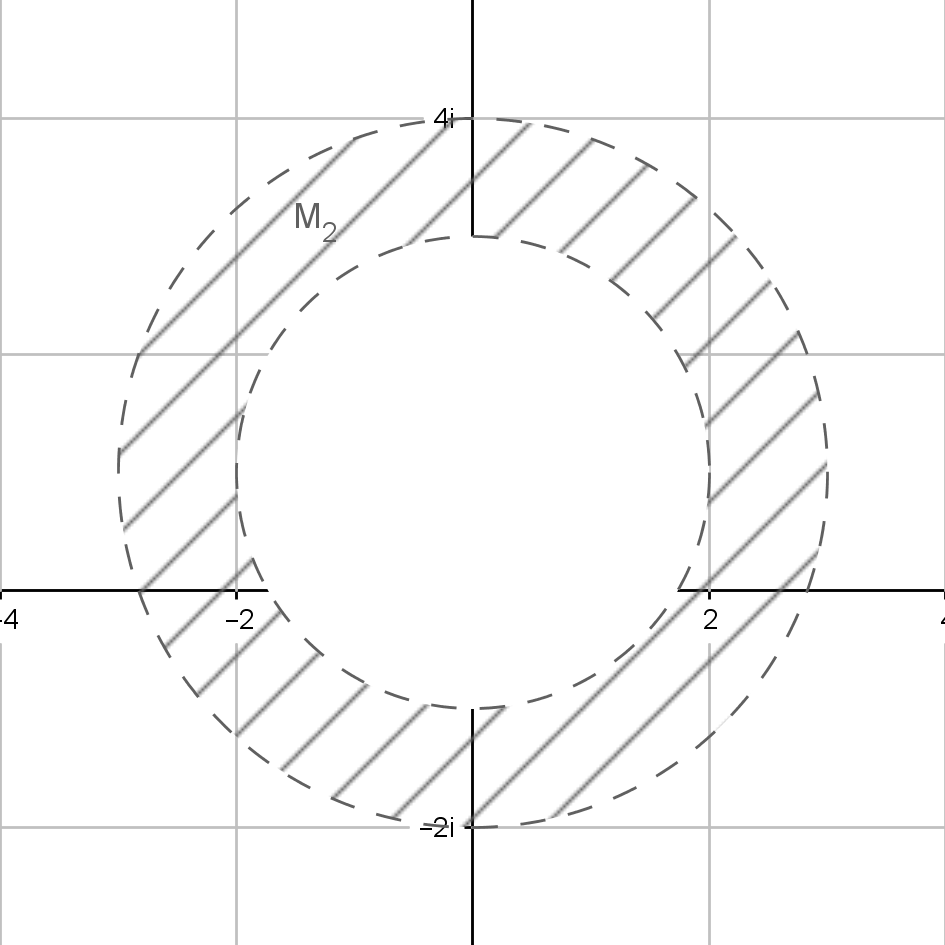
\includegraphics{m2.png}
    \end{figure}
    \end{center}

\item
    $M_3 = \lbrace z \in \CC \mid \vert z \vert \geq 1, \mathrm{Im}(z) > 0, \vert \mathrm{Re}(z) \vert \leq \frac{1}{2}\rbrace$\\ \\
    \begin{center}
    \begin{figure}[ht]
    \centering
    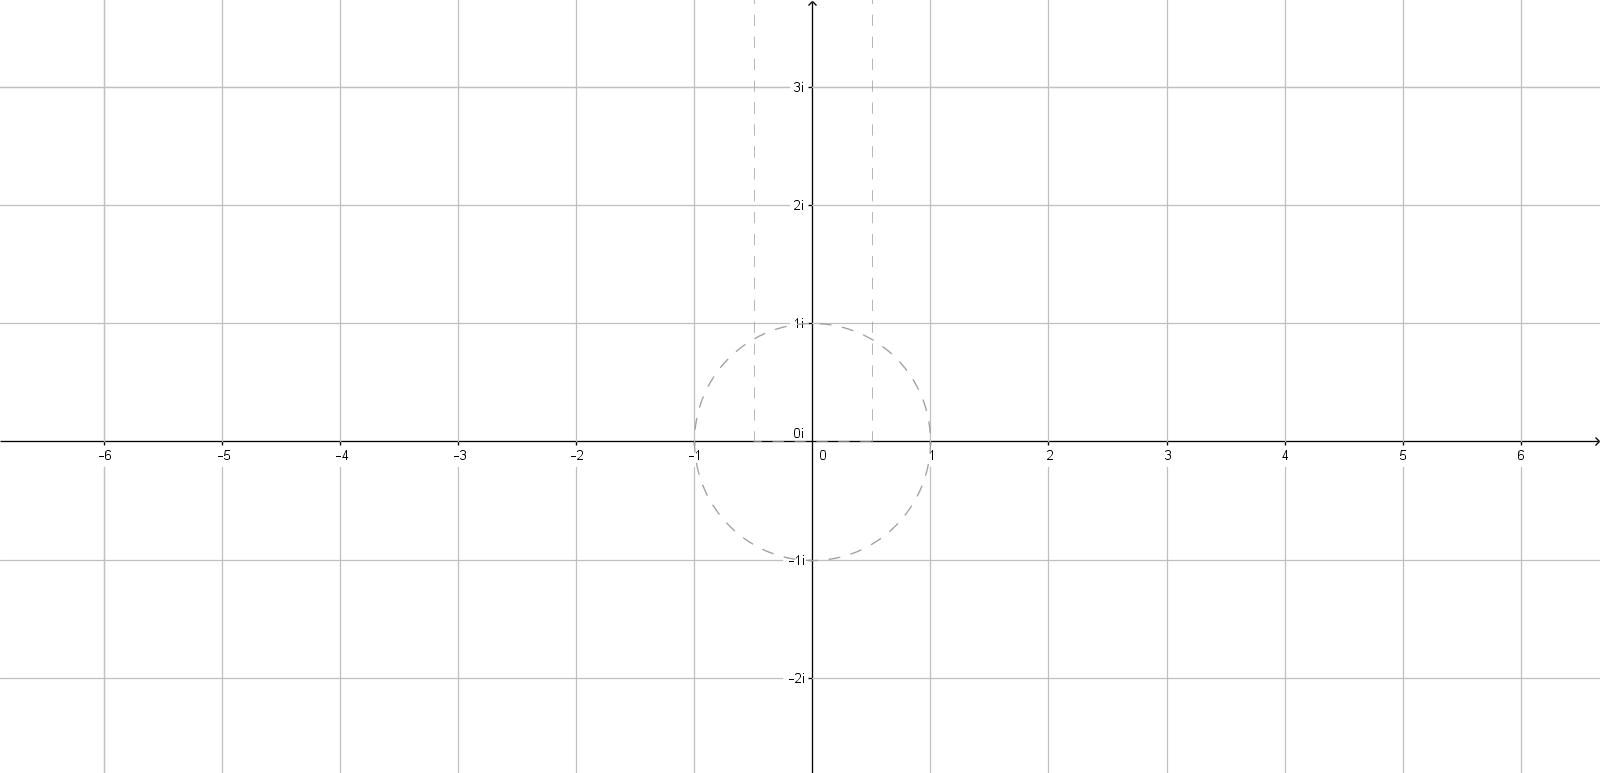
\includegraphics{m3.png}
    \end{figure}
    \end{center}

\end{document}